\section{Datum}
\subsection{Pengertian DATUM}

Datum reference surface atau geodetik atau georeferensi adalah parameter sebagai referensi untuk mendefinisikan geometri Bumi ellipsoid. Datum geodetik diukur menggunakan metode manual agar lebih akurat lagi menggunakan satelit.

Dibawah ini merupakan Jenis geodetik menurut metodenya :
\begin{enumerate}
\item Datum horizontal adalah datum yang digunakan untuk pemetaan horisontal. Dengan teknologi yang lebih maju, kini muncul tren penggunaan datum horizontal dari koordinat geosentris global sebagai penggganti datum lokal atau regional.
\begin{figure}[htbp]
		\centering
		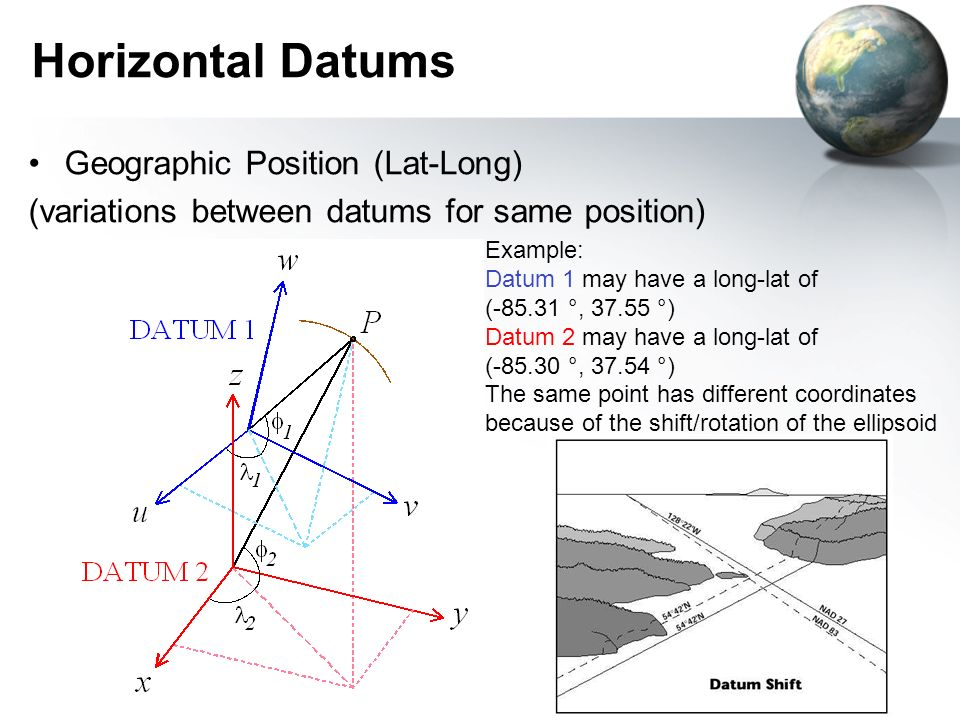
\includegraphics[width=0.75\textwidth]{pictures/datum_horizontal.jpg}
		\caption{Datum Horizontal (Sumber : https://www.slideshare.net/AeroMetri)}
		\label{Datum Horizontal}
		\end{figure}	

\item Datum vertikal adalah sistem referensi untuk ortometris medan tinggi. Datum vertikal digunakan untuk mewakili ketinggian atau kedalaman informasi. Biasanya bidang referensi yang digunakan untuk ortometris sistem tinggi adalah geoid.
\begin{figure}[htbp]
		\centering
		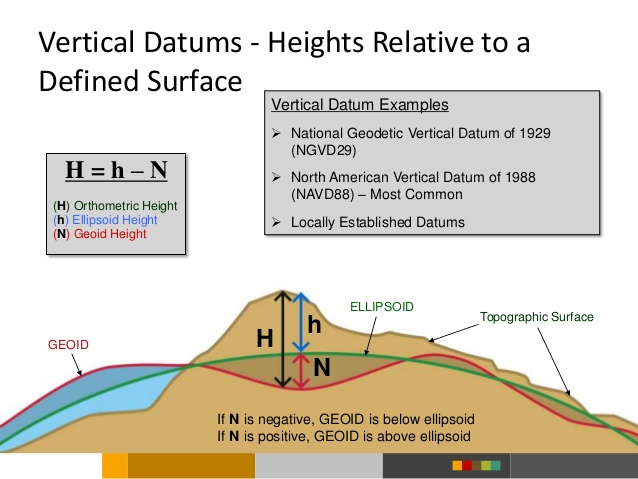
\includegraphics[width=0.75\textwidth]{pictures/vertical_datum.jpg}
		\caption{Datum Vertikal (Sumber : Map Projections and Coordinate Systems 2014)}
		\label{Datum Vertikal}
		\end{figure}	
\end{enumerate}

Sedangkan menurut jenisnya datum geodetik menurut luas areanya :
\begin{enumerate}
\item Datum geodetik lokal adalah bentuk geoid yang paling cocok pada area yang tidak terlalu besar. Sampel datum lokal di Indonesia antara lain: Genoek, datum Monconglowe datum, di 74 (Datum Indonesia 1974), dan dengan 95 (Datum Geodetik Indonesia 1995).
\end{enumerate}